\documentclass[ignorenonframetext, professionalfonts, hyperref={pdftex, unicode}]{beamer}

\usetheme{Copenhagen}
\usecolortheme{wolverine}

%Packages to be included
%\usepackage{graphicx}

\usepackage[russian]{babel}
\usepackage[utf8]{inputenc}
\usepackage[T1]{fontenc}

%%\usepackage[orientation=landscape, size=custom, width=16, height=9.75, scale=0.5]{beamerposter}

\usepackage{textcomp}

\usepackage{beamerthemesplit}

\usepackage{ulem}

\usepackage{verbatim}

\usepackage{ucs}


\usepackage{listings}
\lstloadlanguages{bash}

\lstset{escapechar=`,
	extendedchars=false,
	language=sh,
	frame=single,
	tabsize=2, 
	columns=fullflexible, 
%	basicstyle=\scriptsize,
	keywordstyle=\color{blue}, 
	commentstyle=\itshape\color{brown},
%	identifierstyle=\ttfamily, 
	stringstyle=\mdseries\color{green}, 
	showstringspaces=false, 
	numbers=left, 
	numberstyle=\tiny, 
	breaklines=true, 
	inputencoding=utf8,
	keepspaces=true,
	morekeywords={u\_short, u\_char, u\_long, in\_addr}
	}

\definecolor{darkgreen}{cmyk}{0.7, 0, 1, 0.5}

\lstdefinelanguage{diff}
{
    morekeywords={+, -},
    sensitive=false,
    morecomment=[l]{//},
    morecomment=[s]{/*}{*/},
    morecomment=[l][\color{darkgreen}]{+},
    morecomment=[l][\color{red}]{-},
    morestring=[b]",
}

\author[Epam]{{\bf Epam}\\Low Level Programming Department}

%\institution[EPAM]{EPAM}
%\logo{\includegraphics[width=1cm]{logo.png}}


\title{Введение в GNU/Linux}


%%%%%%%%%%%%%%%%%%%%%%%%%%%%%%%%%%%%%%%%%%%%%%%%%
%%%%%%%%%% Begin Document  %%%%%%%%%%%%%%%%%%%%%%
%%%%%%%%%%%%%%%%%%%%%%%%%%%%%%%%%%%%%%%%%%%%%%%%%




\begin{document}

\frame{
	\frametitle{Дисковая подсистема}
	\titlepage
	\vspace{-0.5cm}
	\begin{center}
	%\frontpagelogo
	\end{center}
}
\frame{
	\tableofcontents
%	[hideallsubsections]
}

%\section{}

\begin{frame}{Дисковая подсистема}

	\begin{block}{Блочное устройство}
		Вид файла устройств в UNIX/Linux-системах,  обеспечивающий интерфейс к устройству,
		реальному или виртуальному, в виде файла в файловой системе.
	\end{block}

	\begin{block}{Файловая система}
		Файловая система определяет формат содержимого и способ физического хранения информации,  
		которую принято группировать в виде файлов. 
		Конкретная файловая система определяет размер имени файла (директории),  
		максимальный возможный размер файла и раздела,  набор атрибутов файла.

		Распространенные для ОС Linux: ext2, ext4, xfs, reiserfs, vfat.
	\end{block}
\end{frame}

\begin{frame}{Примеры блочных устройств}

	\begin{itemize}
		\item {\tt /dev/{\bf s}d*}
		\item {\tt /dev/{\bf h}d*}
		\item {\tt /dev/ram*}
		\item {\tt /dev/loop*}
	\end{itemize}

	\begin{block}{Практическое задание:}
		\begin{enumerate}
			\item Посмотреть список вышеперечисленных устройств
			\item Посмотреть информацию об устройствах {\tt loop0, ram, sda}\\
				Hint: {\tt fdisk -l <device>}
		\end{enumerate}
	\end{block}
\end{frame}

\begin{frame}{Структура диска}
	\begin{columns}
		\column{0.6\textwidth}
		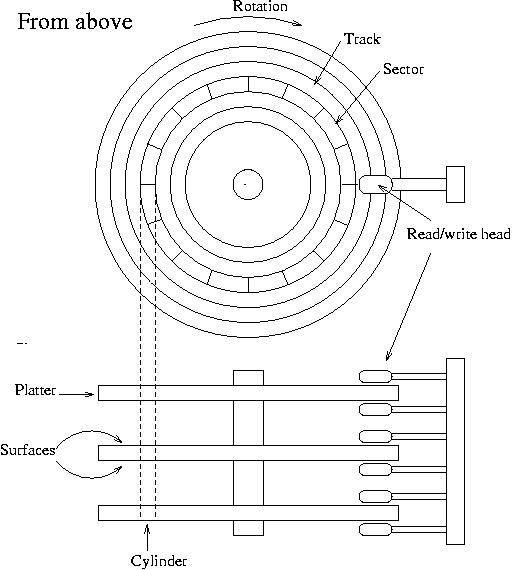
\includegraphics[height=0.8\textheight]{04-hd-schematic.png}
		\column{0.4\textwidth}
		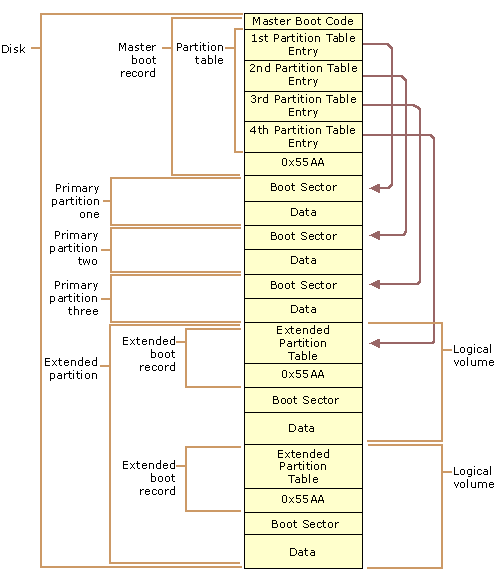
\includegraphics[height=0.8\textheight]{04-disk-structure.png}
	\end{columns}
\end{frame}

\begin{frame}{Отображение блочных устройств}


	\begin{block}{Device Mapper}
			{\tt /dev/mapper/*}\\
			device-mapper -- служит общим фреймворком для отображения одного блочного устройства на другое.

			Примеры: RAID, LVM, шифрованные диски и т.д.
	\end{block}

\end{frame}



\begin{frame}{Полезные утилиты}
	\begin{columns}
		\column{0.25\textwidth}
		\begin{itemize}
			\item {\tt fdisk}
			\item {\tt parted}
			\item {\tt kpartx}
		\end{itemize}
		\column{0.25\textwidth}
		\begin{itemize}
			\item {\tt dd}
			\item {\tt losetup}
		\end{itemize}
		\column{0.25\textwidth}
		\begin{itemize}
			\item {\tt mkfs}
			\item {\tt fsck}
		\end{itemize}
		\column{0.25\textwidth}
		\begin{itemize}
			\item {\tt mount}
			\item {\tt umount}
			\item {\tt df}
		\end{itemize}
	\end{columns}

	\bigskip
	Понадобятся для упражнений:
	\begin{itemize}
			\item[*] {\tt chroot}
			\item[*] {\tt kvm}
	\end{itemize}
\end{frame}


\begin{frame}{Практика: отображение файла на loop-устройство}
	\begin{enumerate}
		\item Создать пустой файл размером 100MB: \\
			dd if=/dev/zero of=test bs=1M count=100
			\pause
		\item Найти неиспользуемое loop-устройство и отобразить на него файл:\\
			losetup -f \\
			losetup loop0 test
			\pause
		\item Посмотреть структуру loop-устройства, создать разделы и посмотреть результаты:\\
			fdisk -l /dev/loop0 \\
			fdisk /dev/loop0 \\
			fdisk -l /dev/loop0
			\pause
		\item Дать команду ядру перечитать разделы и создать устройства для разделов:\\
			ls -l /dev/mapper/* \\
			kpartx -a /dev/loop0 \\
			ls -l /dev/mapper/* \\
	\end{enumerate}
\end{frame}

\begin{frame}{Практика: создание файловой системы}
	\begin{enumerate}
		\item Форматируем файловую систему на устройстве: \\
			mkfs.ext2 /dev/mapper/loop0p1
			\pause
		\item и монтируем:\\
			mkdir -p /mnt/fs\\
			mount\\
			mount /dev/mapper/loop0p1 /mnt/fs\\
			mount\\
			df
			\pause
	\end{enumerate}
\end{frame}


\begin{frame}{Практика: чистимся}
	\begin{enumerate}
		\item Найти смонтированные разделы и отмонтировать их: \\
			mount \\
			umount /dev/mapper/loop0p1
			\pause
		\item Найти используемые loop-устройства\\
			losetup -a \\
			\pause
		\item Корректно удалить устройства для разделов:\\
			ls -l /dev/mapper/* \\
			kpartx -d /dev/loop0 \\
			ls -l /dev/mapper/* \\
			\pause
		\item Удалить отображение файла на loop-устройство: \\
			losetup -d /dev/loop0
	\end{enumerate}
\end{frame}


\begin{frame}{Программный RAID}
  \begin{center}
    \textbf{Уровни RAID поддерживающиеся софтверно}
   \end{center}
   \begin{enumerate}
     \item RAID 0 (длинный диск)
     \pause
     \item RAID 1 (зеркалирование)
     \pause 
     \item RAID 4 (отдельный диск на проверку четности)
     \pause
     \item RAID 5 (данные о четности распределены по дискам)
     \pause
     \item RAID 6 (устойчив при потере двух дисков из 4+)
     \pause
     \item RAID 10 (RAID0 поверх RAID1)
     \pause
     \item RAID 0+1 (RAID1 поверх RAID0)
   \end{enumerate}
   \pause
   Утилита для работы с RAID --\textbf{\tt mdadm}
\end{frame}

\begin{frame}{Упражнения с mdadm}
    \begin{enumerate}
      \item Создать 4 файла по 20Mb из нулей и привязать их к /dev/loop[0-3]
      \item {\tt mdadm -\phantom{}-create /dev/md0 -\phantom{}-level=mirror -\phantom{}-raid-devices=2 /dev/loop0 /dev/loop1}
      \item Создать файловую систему ext3 на /dev/md0. Создать несколько файлов на ней.
      \item {\tt mdadm -\phantom{}-detail /dev/md0}
      \item {\tt mdadm -\phantom{}-manage /dev/md0 -\phantom{}-fault /dev/loop0 } Проверить доступность файловой системы
      \item {\tt mdadm -\phantom{}-manage /dev/md0 -\phantom{}-add /dev/loop2} Проверить доступность файлов на файловой системе
      \item {\tt mdadm -\phantom{}-manage /dev/md0 -\phantom{}-fault /dev/loop1} Проверить доступность
      \item Добавить /dev/loop3
      \item {\tt umount /dev/md0; mdadm -\phantom{}-stop /dev/md0; mdadm -\phantom{}-remove /dev/md0; mdadm -\phantom{}-zero-superblock /dev/loop[0-2]}
    \end{enumerate}
\end{frame}

\begin{frame}{LVM -- управление логическими томами}
  \begin{center}
    \textbf{Структура LVM}
  \end{center}
  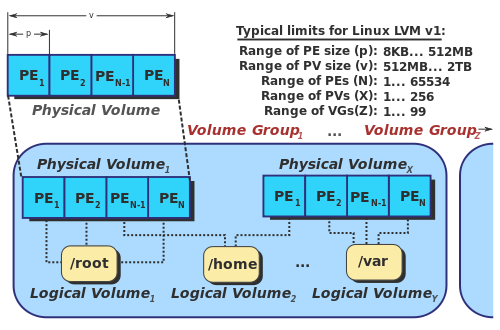
\includegraphics[width=0.7\textwidth]{LVM1-wiki.png}
\end{frame}

\begin{frame}{Преимущества LVM}
	\begin{itemize}
		\item Изменение размера
		\item Перемещение данных в активной системе
		\item Присвоение имен устройствам
		\item Чередование дисков
		\item Зеркалирование томов
		\item Снимки томов
	\end{itemize}
\end{frame}
 
\begin{frame}{LVM -- основные команды}
  \begin{itemize}
    \item Создание
      \begin{columns}
        \column{0.2\textwidth}
        \begin{itemize}
          \item pvcreate
        \end{itemize}
        \column{0.2\textwidth}
        \begin{itemize}
          \item vgcreate
        \end{itemize}
        \column{0.2\textwidth}
        \begin{itemize}
          \item lvcreate
        \end{itemize}
      \end{columns}
     \item Информация 
       \begin{columns}
         \column{0.2\textwidth}
         \begin{itemize}
           \item pvscan
           \item lvscan
           \item vgscan
		   \item lvmdiskscan
         \end{itemize}
         \column{0.2\textwidth}
         \begin{itemize}
           \item pvdisplay
           \item lvdisplay
           \item vgdisplay
		   \item[ ]
         \end{itemize}
         \column{0.2\textwidth}
         \begin{itemize}
           \item pvs
           \item lvs
           \item vgs
		   \item[ ]
         \end{itemize}
	 \end{columns}
      \item Манипулирование
        \begin{itemize}
          \item vgextend/vgreduce
          \item lvresize
          \item pvmove
          \item pvremove
         \end{itemize}
     \end{itemize}
    
\end{frame}

\begin{frame}{Упражнение: создание}
  \begin{enumerate}
    \item Создать 3 файла (200MB) и отобразить на {\tt /dev/loop[0-]}
	\item Найти устройства для работы с LVM {\tt lvmdiskscan}
	\item  {\tt pvcreate /dev/loop[0-2]}
    \item  {\tt pvscan, pvdisplay, pvs}
		\pause
    \item Создание группы томов {\tt vgcreate VG0 /dev/loop[0-2]}
    \item {\tt pvscan, vgscan, pvdisplay}
		\pause
    \item Создание логического тома {\tt lvcreate  -l 50\%VG -i 3 -n lv1 VG0}
	\item Создание файловой системы ext2 на {\tt /dev/VG0/lv1} и монтирование в {\tt /mnt/myfs}
	\end{enumerate}
\end{frame}

\begin{frame}{Изоляция процесса в Linux}
  \begin{center}
    \textbf{В порядке возрастания уровня изоляции}
  \end{center}
  \begin{enumerate}
    \item {\tt chroot}
    \item Linux containers (LXC)
    \item KVM/QEMU
  \end{enumerate}
\end{frame}

\begin{frame}{Упражнение: использование изоляции процесса}
  \begin{block}{chroot}
    \begin{enumerate}
      \item Выбрать из {\tt /media/nfs/pub/soft/linux/emulator/OpenVZ/precreated} систему по вкусу и распаковать {\tt tgz } файл в {\tt /mnt/myfs}
      \item Смонтировать proc и dev файловые системы в новом окружении {\tt /mnt/myfs} \\
		  Hints: {\tt procfs}, опция {\tt -\phantom{}-bind}
      \item {\tt chroot /mnt/myfs /bin/bash}
	  \item {\tt cat /etc/*release}
	  \item {\tt uname -a}
    \end{enumerate}
  \end{block}
\end{frame}

\begin{frame}{Упражнение: Создание снимка LVM}
  \begin{enumerate}
    \item  {\tt lvcreate -\phantom{}-snapshot -l 10\%VG -n snap /dev/VG0/lv1}
    \item  {\tt lvdisplay, lvs, lvscan}
	\item Смонтировать снимок в {\tt /mnt/snap}
		\pause
	\item Удалить директорию {\tt /mnt/snap/etc} или {\tt /mnt/myfs/etc}
	\item Отмонтировать снимок и оригинал\\
		Hint: помним про {\tt proc, dev}
		\pause
	\item Объединяем снимок с оригиналом {\tt lvconvert -\phantom{}-merge VG0/snap}
	\item Монтируем {\tt /dev/VG0/lv1} в {\tt /mnt/myfs} и проверяем изменения
  \end{enumerate}
\end{frame}

\begin{frame}{Упражнение: изменение размера VG}
  \begin{enumerate}
%	\item Отмонтировать {\tt /mnt/myfs}
	\item Создать еще один файл и отобразить его на {\tt loop3}
	\item Увиличиваем размер группы {\tt vgextend VG0 /dev/loop3}
		\pause
    \item  {\tt pvscan; pvmove /dev/loop0; pvscan}
    \item  {\tt vgreduce VG0 /dev/loop0; pvscan}
    \item  {\tt pvremove /dev/loop0; pvscan}
  \end{enumerate}
\end{frame}

\end{document}
